\chapter{Quadrature Phase-Shift Keying (QPSK)}
\label{ch:qpsk}

\begin{nontechnical}
\textbf{QPSK is like using 4 different hand signals instead of 2---you can send messages twice as fast!}

\textbf{Simple idea:}
\begin{itemize}
\item Bits 00 = wave pointing ``northeast'' $\nearrow$ (45°)
\item Bits 01 = wave pointing ``northwest'' $\nwarrow$ (135°)
\item Bits 11 = wave pointing ``southwest'' $\swarrow$ (225°)
\item Bits 10 = wave pointing ``southeast'' $\searrow$ (315°)
\end{itemize}

\textbf{Real use:} Satellite TV (DVB-S), GPS, and 4G LTE all use QPSK. Your phone switches to QPSK when the signal is weak---more reliable than faster modes.

\textbf{Why 4 directions?} Sends 2 bits per symbol (twice as fast as BPSK), but still reliable because the 4 directions are well-separated (90° apart).
\end{nontechnical}

\section{Overview}

\textbf{Quadrature Phase-Shift Keying (QPSK)} is a digital modulation technique that transmits 2 bits per symbol by encoding data into one of four carrier phase states: 45°, 135°, 225°, and 315°.

\begin{keyconcept}
QPSK achieves \textbf{double the spectral efficiency} of BPSK (2~bps/Hz vs 1~bps/Hz) while maintaining the same bit error rate performance at the same $E_b/N_0$. This makes it the optimal choice for bandwidth-limited channels where reliable communication is required.
\end{keyconcept}

QPSK is the foundation for many higher-order modulation schemes including offset QPSK (OQPSK), $\pi$/4-QPSK, and hierarchical QAM constellations.

\section{Mathematical Description}

\subsection{Time-Domain Signal}

The QPSK waveform is expressed as:
\begin{equation}
s(t) = A \cos(2\pi f_c t + \phi_n)
\end{equation}
where:
\begin{itemize}
\item $A$ = carrier amplitude
\item $f_c$ = carrier frequency (Hz)
\item $\phi_n \in \{45°, 135°, 225°, 315°\}$ = phase for symbol $n$
\end{itemize}

\textbf{Phase encoding (Gray coding):}
\begin{equation}
\phi_n = \begin{cases}
45° & \text{if bits = 00} \\
135° & \text{if bits = 01} \\
225° & \text{if bits = 11} \\
315° & \text{if bits = 10}
\end{cases}
\end{equation}

Gray coding ensures adjacent constellation points differ by only one bit, minimizing bit errors when phase noise causes symbol errors.

\subsection{IQ Representation}

The complex baseband representation of QPSK is:
\begin{equation}
s(t) = \mathrm{Re}\left\{A \cdot (I_n + jQ_n) \cdot e^{j2\pi f_c t}\right\}
\end{equation}

Expanding this yields:
\begin{equation}
s(t) = A \cdot I_n \cos(2\pi f_c t) - A \cdot Q_n \sin(2\pi f_c t)
\end{equation}

\textbf{IQ component values for normalized unit-energy symbols:}
\begin{equation}
(I_n, Q_n) = \begin{cases}
(+\frac{1}{\sqrt{2}}, +\frac{1}{\sqrt{2}}) & \text{bits = 00, phase = 45°} \\
(-\frac{1}{\sqrt{2}}, +\frac{1}{\sqrt{2}}) & \text{bits = 01, phase = 135°} \\
(-\frac{1}{\sqrt{2}}, -\frac{1}{\sqrt{2}}) & \text{bits = 11, phase = 225°} \\
(+\frac{1}{\sqrt{2}}, -\frac{1}{\sqrt{2}}) & \text{bits = 10, phase = 315°}
\end{cases}
\end{equation}

\begin{calloutbox}{Physical Interpretation}
QPSK can be viewed as \textbf{two independent BPSK channels} operating in quadrature (90° phase offset). The I-channel modulates $\cos(2\pi f_c t)$ while the Q-channel modulates $\sin(2\pi f_c t)$. This orthogonality allows both channels to occupy the same bandwidth without interference.
\end{calloutbox}

\subsection{Constellation Diagram}

The QPSK constellation consists of four points arranged symmetrically at the corners of a square, separated by 90° in phase:

\begin{center}
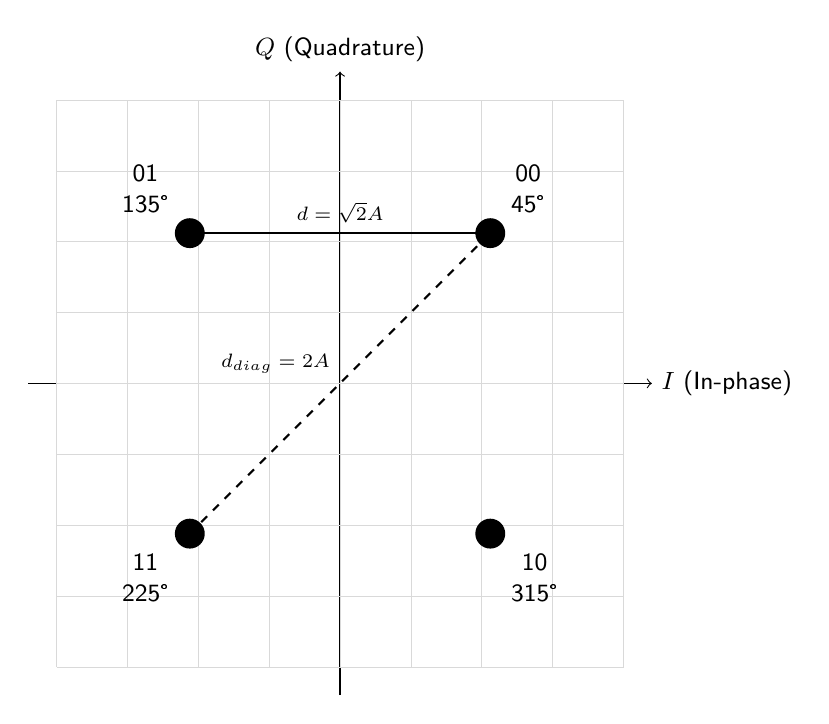
\begin{tikzpicture}[scale=1.8]
% Axes
\draw[->] (-2.2,0) -- (2.2,0) node[right] {\sffamily\small $I$ (In-phase)};
\draw[->] (0,-2.2) -- (0,2.2) node[above] {\sffamily\small $Q$ (Quadrature)};

% Grid
\draw[very thin,gray!30] (-2,-2) grid[step=0.5] (2,2);

% Constellation points
\fill[black] (1.06,1.06) circle (3pt);
\fill[black] (-1.06,1.06) circle (3pt);
\fill[black] (-1.06,-1.06) circle (3pt);
\fill[black] (1.06,-1.06) circle (3pt);

% Bit labels
\node[above right=4pt,align=center,font=\sffamily\small] at (1.06,1.06) {00\\45°};
\node[above left=4pt,align=center,font=\sffamily\small] at (-1.06,1.06) {01\\135°};
\node[below left=4pt,align=center,font=\sffamily\small] at (-1.06,-1.06) {11\\225°};
\node[below right=4pt,align=center,font=\sffamily\small] at (1.06,-1.06) {10\\315°};

% Distance annotation
\draw[<->,thick] (1.06,1.06) -- (-1.06,1.06) node[midway,above,font=\scriptsize] {$d = \sqrt{2}A$};
\draw[<->,thick,dashed] (1.06,1.06) -- (-1.06,-1.06) node[midway,above left,font=\scriptsize] {$d_{diag} = 2A$};
\end{tikzpicture}
\end{center}

\textbf{Key properties:}
\begin{itemize}
\item \textbf{Minimum distance:} $d_{min} = \sqrt{2}A$ (between adjacent points)
\item \textbf{Average symbol energy:} $E_s = A^2 T_s$ where $T_s$ is symbol period
\item \textbf{Gray coding:} Adjacent symbols differ by one bit only
\item \textbf{Equal probability:} All four symbols are equally likely for random data
\end{itemize}

\section{Modulation and Demodulation}

\subsection{Transmitter (Modulator)}

The QPSK modulator splits the input bit stream into two parallel paths (I and Q) and modulates orthogonal carriers:

\begin{center}
\begin{tikzpicture}[
  block/.style={rectangle, draw, minimum width=2.2cm, minimum height=1cm, font=\sffamily\small},
  node distance=2.2cm,
  font=\small
]
\node (input) {\sffamily Binary\\$\{0, 1\}$};
\node[block, right of=input, node distance=2.8cm] (demux) {Serial to\\Parallel};
\node[block, above right of=demux, node distance=2.5cm, yshift=0.5cm] (nrzi) {NRZ\\Map I};
\node[block, below right of=demux, node distance=2.5cm, yshift=-0.5cm] (nrzq) {NRZ\\Map Q};
\node[block, right of=nrzi, node distance=2.8cm] (multi) {Mixer\\$\times$};
\node[block, right of=nrzq, node distance=2.8cm] (multq) {Mixer\\$\times$};
\node[block, right of=multi, node distance=3cm, yshift=-1.5cm] (sum) {Adder\\$+$};
\node[block, right of=sum, node distance=2.5cm] (filter) {Bandpass\\Filter};
\node[right of=filter, node distance=2.8cm] (output) {\sffamily QPSK\\Output};

\node[above of=multi, node distance=1.3cm, font=\scriptsize] (cos) {$\cos(2\pi f_c t)$};
\node[below of=multq, node distance=1.3cm, font=\scriptsize] (sin) {$-\sin(2\pi f_c t)$};

\draw[->,thick] (input) -- (demux);
\draw[->,thick] (demux) -- node[above,font=\scriptsize,pos=0.3] {Even bits} (nrzi);
\draw[->,thick] (demux) -- node[below,font=\scriptsize,pos=0.3] {Odd bits} (nrzq);
\draw[->,thick] (nrzi) -- node[above,font=\scriptsize] {$I_n$} (multi);
\draw[->,thick] (nrzq) -- node[above,font=\scriptsize] {$Q_n$} (multq);
\draw[->,thick] (cos) -- (multi);
\draw[->,thick] (sin) -- (multq);
\draw[->,thick] (multi) -- (sum);
\draw[->,thick] (multq) -- (sum);
\draw[->,thick] (sum) -- (filter);
\draw[->,thick] (filter) -- (output);
\end{tikzpicture}
\end{center}

\textbf{Modulation process:}
\begin{enumerate}
\item \textbf{Serial-to-parallel conversion:} Split bit stream into even (I) and odd (Q) bits
  \begin{itemize}
  \item Even bits (b$_0$, b$_2$, b$_4$, ...) $\rightarrow$ I-channel
  \item Odd bits (b$_1$, b$_3$, b$_5$, ...) $\rightarrow$ Q-channel
  \end{itemize}
\item \textbf{NRZ encoding:} Map bits to bipolar symbols
  \begin{itemize}
  \item Bit 0 $\rightarrow$ $+1/\sqrt{2}$
  \item Bit 1 $\rightarrow$ $-1/\sqrt{2}$
  \end{itemize}
\item \textbf{Carrier multiplication:}
  \begin{align}
  I_{RF}(t) &= I_n \cos(2\pi f_c t) \\
  Q_{RF}(t) &= -Q_n \sin(2\pi f_c t)
  \end{align}
\item \textbf{Summation:} $s(t) = I_{RF}(t) + Q_{RF}(t)$
\item \textbf{Pulse shaping:} Apply raised-cosine filter to limit bandwidth and control ISI
\end{enumerate}

\subsection{Receiver (Coherent Detector)}

\begin{center}
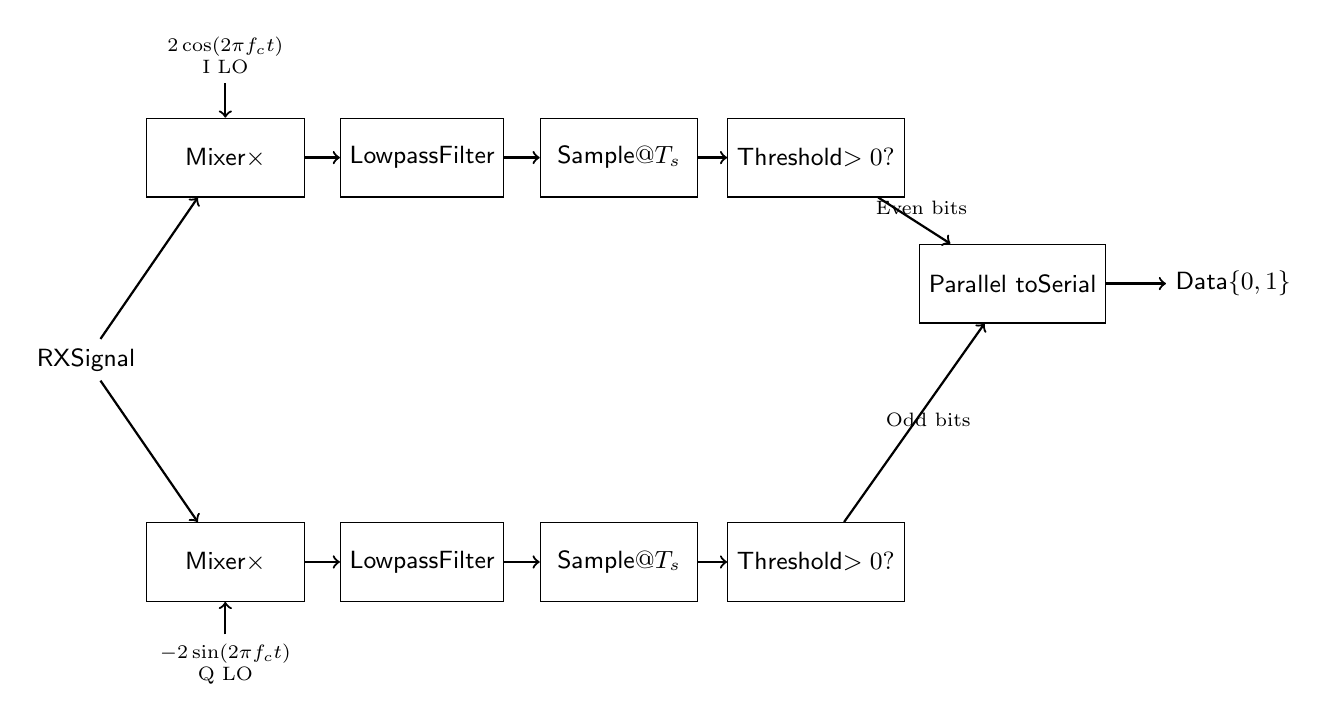
\begin{tikzpicture}[
  block/.style={rectangle, draw, minimum width=2cm, minimum height=1cm, font=\sffamily\small},
  node distance=2cm,
  font=\small
]
\node (input) {\sffamily RX\\Signal};
\node[block, above right of=input, node distance=2.5cm, yshift=0.8cm] (multi) {Mixer\\$\times$};
\node[block, below right of=input, node distance=2.5cm, yshift=-0.8cm] (multq) {Mixer\\$\times$};
\node[block, right of=multi, node distance=2.5cm] (lpfi) {Lowpass\\Filter};
\node[block, right of=multq, node distance=2.5cm] (lpfq) {Lowpass\\Filter};
\node[block, right of=lpfi, node distance=2.5cm] (sampi) {Sample\\$@T_s$};
\node[block, right of=lpfq, node distance=2.5cm] (sampq) {Sample\\$@T_s$};
\node[block, right of=sampi, node distance=2.5cm] (threshi) {Threshold\\$>0?$};
\node[block, right of=sampq, node distance=2.5cm] (threshq) {Threshold\\$>0?$};
\node[block, right of=threshi, node distance=2.5cm, yshift=-1.6cm] (mux) {Parallel to\\Serial};
\node[right of=mux, node distance=2.8cm] (output) {\sffamily Data\\$\{0,1\}$};

\node[above of=multi, node distance=1.3cm, font=\scriptsize, align=center] (cos) {$2\cos(2\pi f_c t)$\\I LO};
\node[below of=multq, node distance=1.3cm, font=\scriptsize, align=center] (sin) {$-2\sin(2\pi f_c t)$\\Q LO};

\draw[->,thick] (input) -- (multi);
\draw[->,thick] (input) -- (multq);
\draw[->,thick] (cos) -- (multi);
\draw[->,thick] (sin) -- (multq);
\draw[->,thick] (multi) -- (lpfi);
\draw[->,thick] (multq) -- (lpfq);
\draw[->,thick] (lpfi) -- (sampi);
\draw[->,thick] (lpfq) -- (sampq);
\draw[->,thick] (sampi) -- (threshi);
\draw[->,thick] (sampq) -- (threshq);
\draw[->,thick] (threshi) -- node[above,font=\scriptsize,pos=0.6] {Even bits} (mux);
\draw[->,thick] (threshq) -- node[below,font=\scriptsize,pos=0.6] {Odd bits} (mux);
\draw[->,thick] (mux) -- (output);
\end{tikzpicture}
\end{center}

\begin{warningbox}
\textbf{Carrier phase and frequency synchronization are critical.} Both I and Q local oscillators must be exactly in phase and frequency with the transmitter carriers. Phase offsets rotate the constellation, potentially causing all symbols to be decoded incorrectly. Carrier recovery circuits (Costas loop) or pilot signals are required.
\end{warningbox}

\textbf{Detection process:}

\begin{enumerate}
\item \textbf{Multiply by in-phase carrier:}
\begin{equation}
r_I(t) = s(t) \cdot 2\cos(2\pi f_c t) = 2I_n \cos^2(2\pi f_c t) - 2Q_n \sin(2\pi f_c t)\cos(2\pi f_c t)
\end{equation}

\item \textbf{Apply trigonometric identities:}
\begin{equation}
r_I(t) = I_n [1 + \cos(4\pi f_c t)] - Q_n \sin(4\pi f_c t)
\end{equation}

\item \textbf{Lowpass filter} removes $2f_c$ components:
\begin{equation}
y_I(t) = I_n + n_I(t)
\end{equation}

\item \textbf{Repeat for quadrature channel} (multiply by $-2\sin(2\pi f_c t)$):
\begin{equation}
y_Q(t) = Q_n + n_Q(t)
\end{equation}

\item \textbf{Sample at symbol period} $T_s$ and make threshold decisions:
\begin{align}
\hat{I}_n &= \begin{cases}
+1 & \text{if } y_I > 0 \quad \text{(decode as bit 0)} \\
-1 & \text{if } y_I < 0 \quad \text{(decode as bit 1)}
\end{cases} \\
\hat{Q}_n &= \begin{cases}
+1 & \text{if } y_Q > 0 \quad \text{(decode as bit 0)} \\
-1 & \text{if } y_Q < 0 \quad \text{(decode as bit 1)}
\end{cases}
\end{align}

\item \textbf{Parallel-to-serial conversion:} Interleave I and Q bit decisions
\end{enumerate}

\section{Bit Error Rate (BER) Performance}

\subsection{QPSK in AWGN Channel}

For ideal coherent detection with perfect synchronization, QPSK achieves the same BER as BPSK:
\begin{equation}
\mathrm{BER} = Q\left(\sqrt{\frac{2E_b}{N_0}}\right) = \frac{1}{2}\mathrm{erfc}\left(\sqrt{\frac{E_b}{N_0}}\right)
\end{equation}
where:
\begin{itemize}
\item $E_b = \frac{E_s}{2} = \frac{A^2 T_s}{2}$ = energy per bit (joules)
\item $E_s = A^2 T_s$ = energy per symbol (joules)
\item $N_0$ = noise power spectral density (W/Hz)
\item $Q(x) = \frac{1}{\sqrt{2\pi}}\int_x^\infty e^{-t^2/2}\,dt$ (Gaussian Q-function)
\end{itemize}

\begin{keyconcept}
\textbf{Why does QPSK have the same BER as BPSK?}

Although QPSK transmits 2 bits per symbol, each bit is detected independently on orthogonal I and Q channels. Since symbol energy $E_s$ is split equally between 2 bits ($E_b = E_s/2$), and the minimum distance is $\sqrt{2}A$, the per-bit error probability matches BPSK while doubling the data rate.
\end{keyconcept}

\textbf{Performance benchmarks:}

\begin{center}
\begin{tabular}{@{}lrl@{}}
\toprule
$E_b/N_0$ (dB) & \multicolumn{1}{c}{BER} & Practical Meaning \\
\midrule
0~dB & $7.9 \times 10^{-2}$ & 1 error in 13 bits \\
5~dB & $9.7 \times 10^{-4}$ & 1 error in 1,000 bits \\
10~dB & $3.9 \times 10^{-6}$ & 1 error in 250,000 bits \\
15~dB & $6.9 \times 10^{-10}$ & 1 error in 1.4 billion bits \\
\bottomrule
\end{tabular}
\end{center}

\subsection{Symbol Error Rate (SER)}

The symbol error rate (probability that the received symbol is decoded incorrectly) is higher than BER:
\begin{equation}
\mathrm{SER} \approx 2Q\left(\sqrt{\frac{2E_b}{N_0}}\right) \left[1 - \frac{1}{2}Q\left(\sqrt{\frac{2E_b}{N_0}}\right)\right]
\end{equation}

At high SNR, this simplifies to:
\begin{equation}
\mathrm{SER} \approx 2 \cdot \mathrm{BER}
\end{equation}

This is because most symbol errors occur at adjacent constellation points (Gray coding), affecting only one bit per symbol error.

\section{Bandwidth Efficiency}

The occupied bandwidth (99\% power) for rectangular pulses is:
\begin{equation}
B \approx \frac{1}{T_s} = \frac{R_b}{2}
\end{equation}
where $R_b$ is the bit rate (bps) and $T_s$ is the symbol period.

With \textbf{raised-cosine pulse shaping} (roll-off factor $\alpha$):
\begin{equation}
B = \frac{R_b}{2}(1 + \alpha)
\end{equation}

\textbf{Typical value:} $\alpha = 0.35$ gives $B = 0.675 R_b$

\textbf{Spectral efficiency:}
\begin{equation}
\eta = \frac{R_b}{B} = \frac{2}{1+\alpha} \approx 1.48\ \text{bps/Hz}
\end{equation}

\begin{calloutbox}{Example: 2~Mbps QPSK System}
\begin{itemize}
\item Data rate: $R_b = 2$~Mbps
\item Symbol rate: $R_s = 1$~Msps (2 bits/symbol)
\item Roll-off: $\alpha = 0.35$
\item Required bandwidth: $B = 1 \times (1 + 0.35) = 1.35$~MHz
\item Spectral efficiency: $\eta = 2/1.35 = 1.48$~bps/Hz
\end{itemize}

\textbf{Comparison to BPSK:} Same 2~Mbps data rate would require 2.7~MHz for BPSK---QPSK uses half the bandwidth!
\end{calloutbox}

\section{Practical Implementations}

\subsection{DVB-S/DVB-S2 Satellite Television}

Digital Video Broadcasting standards use QPSK for reliable long-distance transmission:
\begin{itemize}
\item \textbf{Modulation:} QPSK (DVB-S) or adaptive QPSK/8PSK/16APSK (DVB-S2)
\item \textbf{Frequency:} Ku-band (10.7--12.75~GHz) or Ka-band (18--31~GHz)
\item \textbf{Symbol rate:} 20--45~Msps (typical)
\item \textbf{Data rate:} 40--90~Mbps per transponder
\item \textbf{FEC:} Concatenated Reed-Solomon + Convolutional (DVB-S) or LDPC + BCH (DVB-S2)
\item \textbf{Rationale:} Reliable reception with small dish antennas (45--90~cm) in rain/snow
\end{itemize}

\subsection{GPS Navigation Signals}

Global Positioning System uses BPSK and QPSK for satellite-to-receiver links:
\begin{itemize}
\item \textbf{L1 C/A signal:} BPSK with 1.023~Mcps chipping rate
\item \textbf{L1C/L2C/L5 signals:} QPSK with dual-channel data and pilot
\item \textbf{Carrier frequency:} L1 = 1575.42~MHz, L2 = 1227.60~MHz, L5 = 1176.45~MHz
\item \textbf{Spreading:} Direct-Sequence Spread Spectrum (DSSS) with Gold codes
\item \textbf{Power level:} $-$160~dBW (extremely weak---below thermal noise floor)
\item \textbf{Acquisition:} Correlator-based code phase and Doppler search
\end{itemize}

\subsection{4G LTE Mobile Communications}

Long-Term Evolution uses adaptive modulation including QPSK:
\begin{itemize}
\item \textbf{Uplink:} SC-FDMA with QPSK/16-QAM/64-QAM
\item \textbf{Downlink:} OFDMA with QPSK/16-QAM/64-QAM/256-QAM
\item \textbf{Bandwidth:} 1.4, 3, 5, 10, 15, 20~MHz channels
\item \textbf{Adaptation:} Switch to QPSK at cell edge or in poor signal conditions
\item \textbf{Peak rates:} 3--10~Mbps (QPSK) up to 100--300~Mbps (256-QAM)
\item \textbf{Rationale:} Robustness at low SNR ($<$10~dB $E_b/N_0$)
\end{itemize}

\begin{calloutbox}[colback=black!5!white,colframe=black]{Example: DVB-S2 Link Budget for Europe}
\begin{tabular}{@{}ll@{}}
Satellite TX power & 100~W EIRP = 80~dBW \\
Frequency & 11.5~GHz (Ku-band) \\
Distance & 38,000~km (GEO) \\
RX dish diameter & 60~cm (36~dBi gain) \\
LNB noise figure & 0.8~dB ($T_s \approx 80$~K) \\
Symbol rate & 27.5~Msps \\
\midrule
Free-space path loss & 205.8~dB \\
Received power & $-126$~dBm \\
$C/N_0$ & 77~dB-Hz \\
Required $E_b/N_0$ & 4.5~dB (QPSK + FEC) \\
Link margin & 8~dB \\
\midrule
\textbf{Result} & \textbf{Reliable reception in clear sky} \\
\end{tabular}
\end{calloutbox}

\section{Worked Example: Wireless Microphone Link}

\textbf{Scenario:} Design a QPSK wireless microphone system for theatre production

\subsection*{Given Parameters}

\begin{tabular}{@{}ll@{}}
Audio bandwidth & $B_a = 15$~kHz (high-quality speech) \\
Sampling rate & $f_s = 48$~kHz \\
Quantization & 16 bits/sample \\
RF carrier & $f_c = 2.4$~GHz (ISM band) \\
Available bandwidth & $B_{RF} = 500$~kHz \\
Range & $d = 50$~m (line of sight) \\
TX power & $P_t = 10$~mW = 10~dBm \\
Antenna gain & $G_t = G_r = 2$~dBi (omnidirectional) \\
Required BER & $10^{-6}$ (transparent audio) \\
\end{tabular}

\subsection*{Step 1: Calculate Required Bit Rate}

\begin{equation}
R_b = f_s \times \text{bits/sample} = 48{,}000 \times 16 = 768~\text{kbps}
\end{equation}

\subsection*{Step 2: Add Channel Coding Overhead}

Using rate-1/2 convolutional code for error correction:
\begin{equation}
R_{coded} = 768 \times 2 = 1{,}536~\text{kbps} = 1.536~\text{Mbps}
\end{equation}

\subsection*{Step 3: Calculate Symbol Rate}

For QPSK (2 bits/symbol):
\begin{equation}
R_s = \frac{R_{coded}}{2} = \frac{1{,}536{,}000}{2} = 768~\text{ksps}
\end{equation}

\subsection*{Step 4: Check Bandwidth Requirement}

With raised-cosine pulse shaping ($\alpha = 0.35$):
\begin{equation}
B_{req} = R_s (1 + \alpha) = 768 \times 1.35 = 1{,}037~\text{kHz}
\end{equation}

\textbf{Problem:} Exceeds available 500~kHz! \textbf{Solution:} Use tighter filtering or reduce sample rate.

Revised: Use $\alpha = 0.20$ and 44.1~kHz sampling:
\begin{align}
R_b &= 44{,}100 \times 16 = 705.6~\text{kbps} \\
R_{coded} &= 705.6 \times 2 = 1{,}411.2~\text{kbps} \\
R_s &= 705.6~\text{ksps} \\
B_{req} &= 705.6 \times 1.20 = 847~\text{kHz}
\end{align}

Still too high. Use 32~kHz sampling (broadcast quality):
\begin{align}
R_b &= 32{,}000 \times 16 = 512~\text{kbps} \\
R_{coded} &= 1{,}024~\text{kbps} \\
R_s &= 512~\text{ksps} \\
B_{req} &= 512 \times 1.20 = 614~\text{kHz}
\end{align}

\textbf{Further optimization:} Use 12-bit quantization:
\begin{equation}
B_{req} = \frac{32{,}000 \times 12 \times 2}{2} \times 1.20 = 461~\text{kHz} \quad \checkmark
\end{equation}

\subsection*{Step 5: Link Budget Analysis}

\textbf{Free-space path loss at 2.4~GHz:}
\begin{equation}
\mathrm{FSPL} = 20\log_{10}(50) + 20\log_{10}(2400) + 32.45 = 80.5~\text{dB}
\end{equation}

\textbf{Received power:}
\begin{equation}
P_r = P_t + G_t + G_r - \mathrm{FSPL} = 10 + 2 + 2 - 80.5 = -66.5~\text{dBm}
\end{equation}

\textbf{Noise power (assuming $T_s = 300$~K):}
\begin{equation}
N = kT_sB = (1.38 \times 10^{-23})(300)(461{,}000) = 1.91 \times 10^{-15}~\text{W} = -117~\text{dBm}
\end{equation}

\textbf{SNR:}
\begin{equation}
\mathrm{SNR} = P_r - N = -66.5 - (-117) = 50.5~\text{dB}
\end{equation}

\textbf{$E_b/N_0$:}
\begin{equation}
\frac{E_b}{N_0} = \mathrm{SNR} - 10\log_{10}(B/R_b) = 50.5 - 10\log_{10}(461{,}000/384{,}000) = 49.7~\text{dB}
\end{equation}

\subsection*{Step 6: Verify Link Closure}

\begin{itemize}
\item \textbf{Required $E_b/N_0$ for BER $= 10^{-6}$ (QPSK):} 10.5~dB
\item \textbf{Coding gain (rate-1/2 convolutional):} $\sim$5~dB
\item \textbf{Required $E_b/N_0$ with coding:} 10.5 -- 5 = 5.5~dB
\item \textbf{Available $E_b/N_0$:} 49.7~dB
\item \textbf{Link margin:} $49.7 - 5.5 = 44.2$~dB
\end{itemize}

\begin{calloutbox}[colback=black!8!white,colframe=black]{Design Summary}
\textbf{Result: Link closes with massive 44~dB margin}

This comfortable margin provides:
\begin{itemize}
\item Multipath fading tolerance (20--30~dB)
\item Body shadowing/absorption (5--10~dB)
\item Implementation losses (3--5~dB)
\item Interference margin
\end{itemize}

\textbf{Final design:}
\begin{itemize}
\item Modulation: QPSK
\item Sample rate: 32~kHz, 12-bit
\item Data rate: 768~kbps (384~kbps after FEC)
\item Symbol rate: 384~ksps
\item Bandwidth: 461~kHz
\item Link margin: 44~dB
\end{itemize}

\textbf{Conclusion:} Design is viable with significant margin for real-world impairments.
\end{calloutbox}

\section{Advantages and Disadvantages}

\subsection*{Advantages}

\begin{enumerate}
\item \textbf{Double spectral efficiency:} 2~bps/Hz vs 1~bps/Hz for BPSK (twice data rate in same bandwidth)
\item \textbf{Same BER as BPSK:} No performance penalty at same $E_b/N_0$
\item \textbf{Constant envelope:} Compatible with nonlinear amplifiers (Class C, Class D)
\item \textbf{Mature technology:} Well-understood with extensive commercial implementations
\item \textbf{Gray coding:} Most symbol errors affect only one bit, minimizing BER
\item \textbf{Power efficient:} Optimal for bandwidth-limited channels requiring reliable links
\end{enumerate}

\subsection*{Disadvantages}

\begin{enumerate}
\item \textbf{Carrier synchronization required:} Costas loop or pilot signals add complexity and overhead
\item \textbf{Phase ambiguity:} 90° rotations of constellation require differential encoding or unique word sync
\item \textbf{Lower spectral efficiency than QAM:} 16-QAM achieves 4~bps/Hz but requires higher SNR
\item \textbf{Susceptible to phase noise:} Oscillator stability critical for maintaining constellation alignment
\item \textbf{Fixed data rate:} Cannot adapt modulation depth (unlike adaptive QAM schemes)
\end{enumerate}

\section{Summary}

\begin{center}
\begin{tabular}{@{}ll@{}}
\toprule
\textbf{Parameter} & \textbf{Value} \\
\midrule
Bits per symbol & 2 \\
Constellation points & 4 (45°, 135°, 225°, 315°) \\
Spectral efficiency & $\sim$1.4--2.0~bps/Hz \\
BER @ 10~dB $E_b/N_0$ & $3.9 \times 10^{-6}$ \\
Minimum phase separation & 90° \\
Symbol energy & $E_s = 2E_b$ \\
Carrier recovery & Required (Costas loop or pilot) \\
Implementation & Moderate complexity (I/Q channels) \\
Best application & Bandwidth-limited reliable links \\
Typical uses & Satellite TV, GPS, LTE, WiFi \\
\bottomrule
\end{tabular}
\end{center}

\vspace{10pt}

\textbf{Key takeaways:}
\begin{itemize}
\item QPSK doubles spectral efficiency over BPSK with no BER penalty
\item Requires carrier synchronization but offers excellent power efficiency
\item Widely deployed in satellite, terrestrial wireless, and navigation systems
\item Foundation for higher-order PSK and QAM modulation schemes
\end{itemize}

\section{Further Reading}

\subsection*{Related Chapters}

\begin{itemize}
\item \textbf{Chapter~\ref{ch:bpsk}:} Binary Phase-Shift Keying (BPSK)---foundation for QPSK
\item \textbf{Chapter 8:} Offset QPSK (OQPSK)---reduced envelope variation
\item \textbf{Chapter 9:} $\pi$/4-DQPSK---differential QPSK with rotation
\item \textbf{Chapter 10:} 8PSK and 16PSK---higher-order phase modulation
\item \textbf{Chapter 11:} Quadrature Amplitude Modulation (QAM)---combined amplitude/phase
\item \textbf{Chapter 12:} Constellation Diagrams---visualization techniques
\item \textbf{Chapter 13:} IQ Representation---complex baseband mathematics
\item \textbf{Chapter 18:} Bit Error Rate Analysis---performance measurement
\item \textbf{Chapter 22:} Forward Error Correction---coding for BER improvement
\item \textbf{Chapter 25:} Carrier Recovery Techniques---Costas loop and alternatives
\end{itemize}

\subsection*{Standards and References}

\begin{itemize}
\item ETSI EN 302 307: \textit{Digital Video Broadcasting (DVB-S2)}
\item IS-GPS-200: \textit{GPS Interface Specification}
\item 3GPP TS 36.211: \textit{LTE Physical Channels and Modulation}
\item IEEE 802.11: \textit{Wireless LAN QPSK/OFDM}
\item Proakis \& Salehi: \textit{Digital Communications}, Chapter 4
\end{itemize}
